% Corazón v2 — diapositivas de la sustentación (MIA-203, Grupo 6). 20 diapositivas, 25 min.
% Compilar desde slides/: pdflatex slides (dos veces). Figuras: python slides/figuras.py desde la raíz del repo.
% Cada número sale de results/ (el mismo archivo que cita paper/main.tex).
\documentclass[aspectratio=169,11pt]{beamer}
\usepackage[utf8]{inputenc}
\usepackage[T1]{fontenc}
\usepackage{lmodern}
\usepackage[spanish,es-noshorthands,es-tabla,es-nodecimaldot]{babel}
\usepackage{amsmath}
\usepackage{booktabs}
\usepackage{array}
\usepackage{tikz}
\usetikzlibrary{positioning,arrows.meta}

% --- Estilo -----------------------------------------------------------------------------------------------------------
\definecolor{tinta}{HTML}{1F2328}
\definecolor{tinta2}{HTML}{57606A}
\definecolor{medir}{HTML}{2A78D6}
\definecolor{clasif}{HTML}{EB6834}
\definecolor{linea}{HTML}{D8DEE4}
\definecolor{fondo2}{HTML}{F4F6F8}
\setbeamercolor{normal text}{fg=tinta,bg=white}
\setbeamercolor{frametitle}{fg=tinta}
\setbeamercolor{structure}{fg=medir}
\setbeamercolor{alerted text}{fg=clasif}
\setbeamerfont{frametitle}{size=\Large,series=\bfseries}
\setbeamertemplate{navigation symbols}{}
\setbeamertemplate{itemize items}{\raisebox{0.15em}{\tikz\fill[medir] (0,0) circle (0.22em);}}
\setbeamertemplate{frametitle}{\vspace{0.6em}\insertframetitle\par\vspace{-0.15em}
  {\color{medir}\rule{2.2em}{2pt}}\vspace{-0.3em}}
\setbeamertemplate{footline}{\hfill{\color{tinta2}\scriptsize Corazón v2 · Grupo 6 · \insertframenumber/\inserttotalframenumber}\hspace{1.2em}\vspace{0.7em}}
\newcommand{\bloque}[1]{{\color{tinta2}\footnotesize\textsc{#1}}\par\vspace{0.1em}}
\newcommand{\cifra}[2]{{\color{#1}\fontsize{26}{28}\selectfont\bfseries #2}}
\newcommand{\nota}[1]{{\color{tinta2}\footnotesize #1}}
\newcommand{\M}[1]{{\color{medir}\bfseries #1}}
\newcommand{\C}[1]{{\color{clasif}\bfseries #1}}

\begin{document}

% ======================================================================================================================
% Portada
\begin{frame}[plain]
\vspace{1.2em}
{\color{tinta2}\small Universidad Nacional de Ingeniería · FIIS · Maestría en Inteligencia Artificial\\
MIA-203 Redes Neuronales y Aprendizaje Profundo · Examen final}

\vspace{1.4em}
{\fontsize{28}{32}\selectfont\bfseries Medir como el radiólogo}\\[0.4em]
{\Large Índice cardiotorácico con \M{U-Net} frente a una \C{CNN de caja negra}\\ para detectar cardiomegalia}

\vspace{1.6em}
{\color{medir}\rule{3em}{2pt}}\\[0.6em]
\textbf{Grupo 6}\\[0.2em]
\small Juan Sebastian Contreras Avendaño · Junior Francesco Romero Lovera · Luis Muñoz Cañabe\\
Derly Raúl Oha Quispe · Lourdes Pedraza Palomino

\vfill
\nota{Lima, 7 de noviembre de 2026 · github.com/loupv99/corazon-v2}
\end{frame}

% ======================================================================================================================
% Bloque 1 — Problema, motivación y contribuciones (3 min)
\begin{frame}{El problema: ¿el corazón está agrandado?}
\bloque{Problema y motivación}
\begin{columns}[T]
\begin{column}{0.55\textwidth}
\begin{itemize}
\item La cardiomegalia se sospecha con el \textbf{índice cardiotorácico}:
\[\text{ICT}=\frac{\text{ancho del corazón}}{\text{ancho interno del tórax}}\]
\item \textbf{ICT $>$ 0.50} en placa PA sugiere cardiomegalia.
\item Es una \emph{medida}: el radiólogo traza líneas y divide. Sin radiólogo, la placa espera.
\item Dos caminos con aprendizaje profundo: \M{medir} el ICT con contornos o \C{clasificar} la placa entera.
\end{itemize}
\end{column}
\begin{column}{0.4\textwidth}
\centering
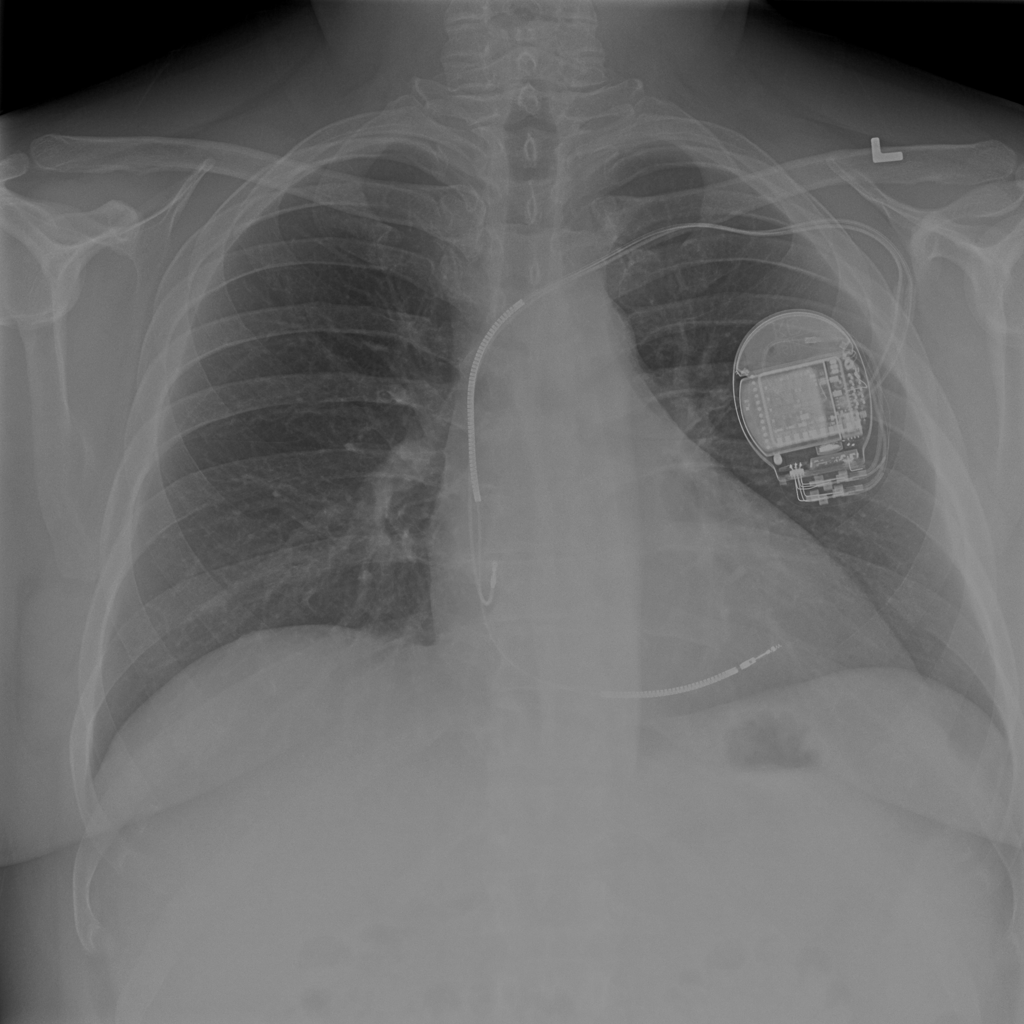
\includegraphics[height=0.62\textheight]{../app/ejemplos/con_cardiomegalia.png}\\
\nota{Placa de prueba de ChestX-ray14 (NIH)}
\end{column}
\end{columns}
\end{frame}

\begin{frame}{Pregunta y contribuciones}
\bloque{Problema y motivación}
\begin{center}
{\large ¿Una red que \M{mide} como el radiólogo detecta tan bien\\como una red que \C{clasifica} sin explicar? ¿Y cuál falla mejor?}
\end{center}
\vspace{0.6em}
\begin{enumerate}
\item \textbf{Comparación controlada medir frente a clasificar}, con las mismas particiones y 3 semillas: U-Net
  entrenada con \emph{máscaras automáticas} (CheXmask) y evaluada contra \emph{contornos humanos} (SCR).
\item \textbf{El atajo de la proyección AP}, medido en ambos enfoques, con una corrección explícita para el ICT y
  Grad-CAM para la caja negra.
\item \textbf{Un conjunto de datos propio}: 300 fotos con celular de 100 radiografías, con marcas ArUco para
  enderezarlas, y una \textbf{aplicación web} que mide el ICT en el teléfono y deja corregir la medida.
\end{enumerate}
\end{frame}

% ======================================================================================================================
% Bloque 2 — Trabajos relacionados y fundamento teórico (3 min)
\begin{frame}{Trabajos relacionados}
\bloque{Trabajos relacionados}
\footnotesize\renewcommand{\arraystretch}{1.25}
\begin{tabular}{@{}>{\raggedright}p{0.25\textwidth}>{\raggedright}p{0.33\textwidth}>{\raggedright\arraybackslash}p{0.36\textwidth}@{}}
\toprule
Trabajo & Qué hace & En qué nos diferenciamos \\
\midrule
Ronneberger 2015 · U-Net & Codificador-decodificador con saltos & La usamos para medir, no solo segmentar \\
He 2016 · ResNet & Conexiones residuales & Línea base de caja negra \\
Selvaraju 2017 · Grad-CAM & Mapa de dónde mira la red & Lo cuantificamos por acierto y error \\
Sogancioglu 2020 & Segmentación vs.\ clasificación & Máscaras \emph{automáticas}, vista AP, fotos \\
Chamveha 2020 & ICT como MRD + MLD & Cada lado por separado (E6) \\
Gaggion 2022, 2024 · HybridGNet, CheXmask & Máscaras con una red de grafos & Las destilamos en una U-Net ligera \\
Zech 2018 · CheXphoto 2020 & Atajos de hospital; fotos de placas & Ambos efectos sobre una \emph{medida} \\
\bottomrule
\end{tabular}
\end{frame}

\begin{frame}{Fundamento: por qué estas dos arquitecturas}
\bloque{Fundamento teórico}
\begin{columns}[T]
\begin{column}{0.48\textwidth}
\M{U-Net — medir}
\begin{itemize}
\item El codificador baja a 1/16 para ver contexto; los \textbf{saltos} devuelven el detalle del borde.
\item El ICT depende de bordes exactos: un error de 3 px en 256 cambia el ICT en $\sim$0.01.
\item Sigmoide por canal: el corazón se superpone a los pulmones.
\item Salida \textbf{verificable}: contornos que el médico ve.
\end{itemize}
\end{column}
\begin{column}{0.48\textwidth}
\C{ResNet-50 — clasificar}
\begin{itemize}
\item Bloques residuales $y=F(x)+x$: profundidad sin degradación.
\item Preentrenada en ImageNet: buen punto de partida con 5\,416 placas.
\item Ve toda la placa: puede usar señales que el ICT ignora… y atajos.
\item Grad-CAM: $\;L=\mathrm{ReLU}\big(\sum_k \alpha_k A^k\big)$,\\ $\alpha_k=\frac{1}{Z}\sum_{i,j}\frac{\partial y}{\partial A^k_{ij}}$
\end{itemize}
\end{column}
\end{columns}
\end{frame}

% ======================================================================================================================
% Bloque 3 — Datos y metodología (6 min)
\begin{frame}{Datos: tres fuentes, una partición sin fuga}
\bloque{Datos}
\begin{columns}[T]
\begin{column}{0.55\textwidth}
\small
\begin{tabular}{lrrr}
\toprule
ChestX-ray14 & Placas & Cardio. & AP \\
\midrule
Entrenamiento & 5\,416 & 1\,471 & 1\,829 \\
Validación & 1\,006 & 236 & 357 \\
Prueba (oficial NIH) & 2\,354 & 1\,069 & 1\,335 \\
\bottomrule
\end{tabular}

\vspace{0.6em}
\begin{itemize}
\item Partición por \textbf{paciente} (5\,674): nadie aparece en dos particiones.
\item Negativos con y sin otros hallazgos: la red no aprende ``sano vs.\ enfermo''.
\item \alert{La vista está asociada a la etiqueta}: 43.7\,\% AP en cardiomegalia frente a 38.5\,\% sin ella.
\end{itemize}
\end{column}
\begin{column}{0.4\textwidth}
\small
\textbf{CheXmask} (CC BY 4.0)\\ máscaras \emph{automáticas} de pulmones y corazón para las 8\,776 placas; 8\,666 con
calidad RCA $\geq$ 0.7.

\vspace{0.6em}
\textbf{SCR / JSRT} (CC BY 4.0)\\ contornos \emph{humanos} en 247 placas: 147 de prueba dorada, 80 + 20 para ajuste
fino.

\vspace{0.6em}
\textbf{Fotos propias}\\ 300 fotos de 100 placas de prueba con dos celulares.
\end{column}
\end{columns}
\end{frame}

\begin{frame}{Etiquetas débiles, referencia humana}
\bloque{Datos}
\centering
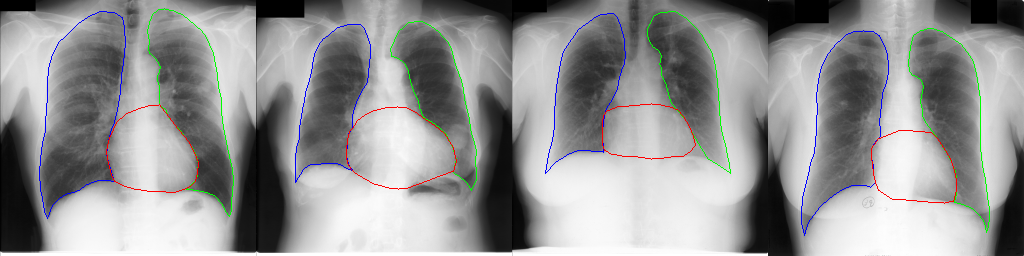
\includegraphics[width=0.92\textwidth]{../results/kaggle-v1/control_scr.png}\\[0.4em]
\nota{Contornos humanos de SCR rasterizados (azul: pulmón derecho; verde: izquierdo; rojo: corazón)}
\vspace{0.6em}
\begin{itemize}
\item La U-Net \textbf{aprende} de máscaras de HybridGNet (convoluciones + red de grafos) y se \textbf{evalúa} en
  contornos trazados por personas: una destilación hacia una red que cabe en un navegador.
\item Sin volteo horizontal en el aumento: el corazón está a la izquierda del paciente.
\end{itemize}
\end{frame}

\begin{frame}{Arquitectura del sistema}
\bloque{Metodología}
\centering
\begin{tikzpicture}[font=\small, node distance=5mm and 6mm,
  caja/.style={draw=linea, fill=fondo2, rounded corners=3pt, align=center, inner sep=4pt, minimum height=11mm, text width=26mm},
  flecha/.style={-{Stealth[length=2.5mm]}, thick, color=tinta2}]
\node[caja] (x) {Radiografía\\$1\times256\times256$};
\node[caja, right=of x, yshift=9mm, draw=medir] (u) {\textbf{U-Net}\\7.8\,M parámetros\\desde cero};
\node[caja, right=of u] (m) {3 máscaras\\pulmones D e I,\\corazón};
\node[caja, right=of m, draw=medir] (ict) {MRD, MLD, ID\\$\Rightarrow$ \textbf{ICT}};
\node[caja, right=of x, yshift=-9mm, draw=clasif] (r) {\textbf{ResNet-50}\\23.5\,M parám.\\preentrenada};
\node[caja, right=of r] (p) {$p$(cardiomegalia)};
\node[caja, right=of p, draw=clasif] (g) {\textbf{Grad-CAM}\\sobre layer4};
\draw[flecha] (x) -- (u); \draw[flecha] (u) -- (m); \draw[flecha] (m) -- (ict);
\draw[flecha] (x) -- (r); \draw[flecha] (r) -- (p); \draw[flecha] (p) -- (g);
\end{tikzpicture}

\vspace{1em}
\begin{columns}[T]
\begin{column}{0.47\textwidth}\small
\M{U-Net}: 4 niveles (32--256 canales) + cuello de 512; cada bloque = 2 × (conv $3\times3$, BatchNorm, ReLU);
sube con conv. transpuesta y concatena el salto; salida $1\times1$ con 3 sigmoides.
\end{column}
\begin{column}{0.47\textwidth}\small
\C{ResNet-50}: capa final cambiada por una salida; gris repetido en 3 canales; mismas imágenes, partición y aumento
que la U-Net.
\end{column}
\end{columns}
\end{frame}

\begin{frame}{Formulación: pérdida y medida}
\bloque{Metodología}
\begin{columns}[T]
\begin{column}{0.5\textwidth}
\M{Segmentación}: BCE + Dice promediado por canal
\[\mathcal{L}_{\text{seg}}=\text{BCE}(\hat y,y)+1-\frac13\sum_{c=1}^{3}\frac{2\sum_i\hat y_{c,i}y_{c,i}+\epsilon}{\sum_i\hat y_{c,i}+\sum_i y_{c,i}+\epsilon}\]
\nota{El promedio por canal evita que los pulmones, más grandes, dominen al corazón.}

\vspace{0.8em}
\C{Clasificación}: BCE con peso $w_+=N_-/N_+$
\[\mathcal{L}_{\text{cls}}=-\frac1N\sum_n\big[w_+y_n\log p_n+(1-y_n)\log(1-p_n)\big]\]
\end{column}
\begin{column}{0.46\textwidth}
\M{Del contorno al número}
\begin{itemize}
\item Umbral 0.5 y mayor componente conexa.
\item ID: la fila más ancha entre bordes externos de los pulmones; su centro es la línea media $x_m$.
\item $\text{MRD}=x_m-x_{\min}$, \ $\text{MLD}=x_{\max}-x_m$
\[\text{ICT}=\frac{\text{MRD}+\text{MLD}}{\text{ID}}\]
\item Si falta una estructura: \emph{no medible}.
\end{itemize}
\end{column}
\end{columns}
\end{frame}

\begin{frame}{Entrenamiento y costo}
\bloque{Metodología}
\begin{columns}[T]
\begin{column}{0.56\textwidth}
\small
\begin{tabular}{lccc}
\toprule
& U-Net & Ajuste E1c & ResNet-50 \\
\midrule
Épocas & 30 & 30 & 12 \\
Lote & 16 & 8 & 32 \\
Tasa máx. & $10^{-3}$ & $2\times10^{-4}$ & $3\times10^{-4}$ \\
Elige época por & Dice val. & Dice 20 humanas & AUC val. \\
\bottomrule
\end{tabular}

\vspace{0.4em}
\nota{AdamW (decaimiento $10^{-4}$), OneCycle, precisión mixta. Aumento: rotación $\pm10^\circ$, escala 0.9--1.1,
traslación $\pm5$\,\%, brillo/contraste $\pm15$\,\%.}
\end{column}
\begin{column}{0.4\textwidth}
\begin{itemize}
\item \textbf{3 semillas} (0, 1, 2): media $\pm$ D.\,E.
\item Umbral ResNet: Youden en validación. ICT: \textbf{0.50 clínico}, sin ajustar.
\item La prueba no se usó para elegir nada.
\end{itemize}
\vspace{0.4em}
\cifra{tinta}{4.2 h} \ {\small de GPU}\\
\nota{Kaggle, 2 × Tesla T4. E5 y E6 en el CPU de una laptop (E5: 35.5 min).}
\end{column}
\end{columns}
\end{frame}

\begin{frame}{Diseño experimental}
\bloque{Metodología}
\small
\begin{tabular}{p{0.2\textwidth}p{0.4\textwidth}p{0.3\textwidth}}
\toprule
Experimento & Qué se compara & Métrica \\
\midrule
E1 Ablación de etiquetas & Débiles todas / filtradas RCA $\geq$ 0.7 / + 80 humanas & Dice en SCR \\
E2 Línea base & ICT U-Net, ResNet-50, ICT de CheXmask sin red, reg.\ log.\ [ICT, vista] & AUC, sens., esp., F1 \\
E3 Acuerdo clínico & ICT de la U-Net vs.\ ICT de contornos humanos & ICC(A,1), Bland-Altman \\
E4 Proyección & AUC por vista; ResNet solo PA; fuga de vista; Grad-CAM & AUC PA/AP, fuga \\
E5 Fotos & Original vs.\ 3 condiciones reales + 6 sintéticas & \% de decisiones que cambian, AUC \\
E6 Lado derecho & MRD/ID y MLD/ID por separado & AUC, aciertos vs.\ errores \\
\bottomrule
\end{tabular}

\vspace{0.6em}
\nota{Fuga de vista = AUC del puntaje para separar AP de PA \emph{solo entre placas sin cardiomegalia}; 0.5 = el
puntaje no codifica la vista.}
\end{frame}

% ======================================================================================================================
% Bloque 4 — Resultados (7 min)
\begin{frame}{Resultado 1: la caja negra detecta mejor}
\bloque{Resultados · línea base}
\begin{columns}[c]
\begin{column}{0.62\textwidth}
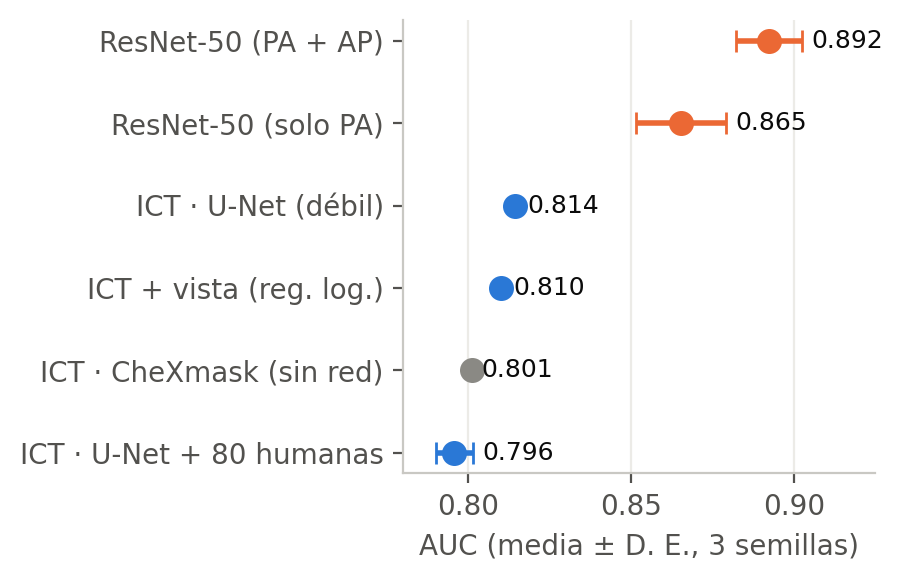
\includegraphics[width=\textwidth]{figs/auc_metodos.png}
\end{column}
\begin{column}{0.35\textwidth}
\begin{itemize}
\item \C{ResNet-50}: AUC \textbf{0.892}, en las 3 semillas y en ambas vistas.
\item \M{ICT}: \textbf{0.814}; supera al ICT de CheXmask sin red (0.801).
\item Al umbral 0.50: sens.\ 0.918, esp.\ 0.504.
\item El umbral no es el problema: Youden en validación = 0.495--0.497.
\end{itemize}
\end{column}
\end{columns}
\end{frame}

\begin{frame}{Resultado 2: mide bien, aun sin contornos humanos}
\bloque{Resultados · ablación y acuerdo clínico}
\begin{center}\small
\begin{tabular}{lcccc}
\toprule
Variante (147 placas SCR) & Dice corazón & Dice medio & Error ICT & ICC(A,1) \\
\midrule
E1a débil, todas & 0.936 & 0.962 & 0.012 & 0.948--0.953 \\
E1b débil, RCA $\geq$ 0.7 & 0.936 & 0.961 & 0.012 & 0.945--0.951 \\
E1c E1b + 80 humanas & \textbf{0.951} & \textbf{0.971} & \textbf{0.010} & \textbf{0.964--0.971} \\
\bottomrule
\end{tabular}
\end{center}
\vspace{0.3em}
\begin{columns}[T]
\begin{column}{0.48\textwidth}
\begin{itemize}
\item Filtrar por calidad no cambia nada: solo 110 de 8\,776 máscaras bajo RCA 0.7.
\item E1c: sesgo de $-0.0035$ a $-0.0005$; Bland-Altman $\approx\pm0.03$.
\end{itemize}
\end{column}
\begin{column}{0.48\textwidth}
\alert{Paradoja}: E1c mide mejor, pero su AUC baja de 0.814 a \textbf{0.796}.\\
\nota{Medir mejor no es diagnosticar mejor cuando la etiqueta no es la medida. Además, la mejora se mide en JSRT,
el mismo dominio del ajuste.}
\end{column}
\end{columns}
\end{frame}

\begin{frame}{Resultado 3: el atajo de la proyección AP}
\bloque{Resultados · comparación controlada}
\begin{columns}[c]
\begin{column}{0.6\textwidth}
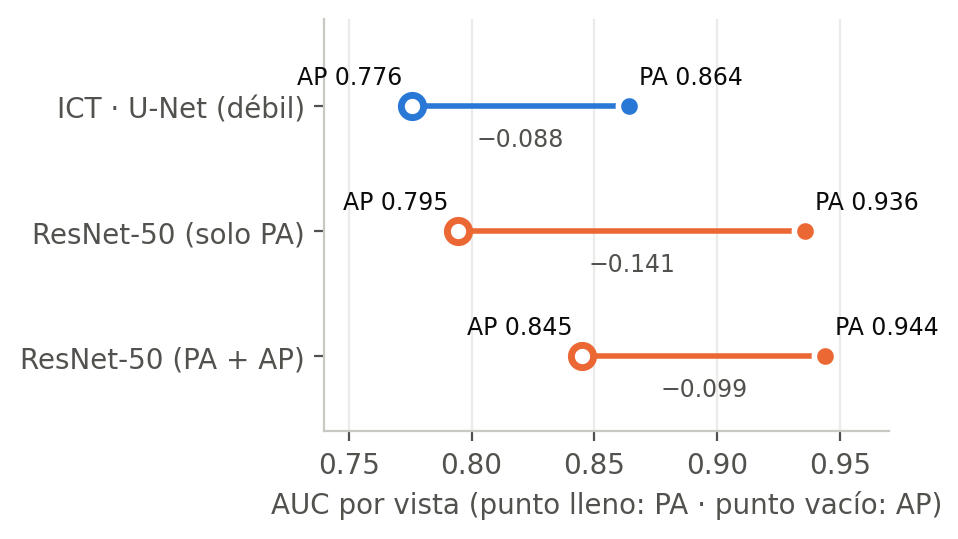
\includegraphics[width=\textwidth]{figs/vista_pa_ap.png}
\end{column}
\begin{column}{0.37\textwidth}
\small
\begin{itemize}
\item Todos pierden en AP. La ResNet que solo vio PA pierde \textbf{0.141}.
\item La ResNet \C{codifica la vista}: fuga 0.646 (0.710 solo PA).
\item En el \M{ICT} la causa es física (magnificación): esp.\ AP = 0.356.
\item \M{Corrección con la vista} (reg.\ log.): fuga \textbf{0.691 $\to$ 0.493}, esp.\ AP \textbf{0.356 $\to$ 0.619},
  a costa de 0.004 de AUC.
\end{itemize}
\end{column}
\end{columns}
\end{frame}

\begin{frame}{Resultado 4: 300 fotos con celular}
\bloque{Resultados · datos propios}
\begin{columns}[c]
\begin{column}{0.4\textwidth}
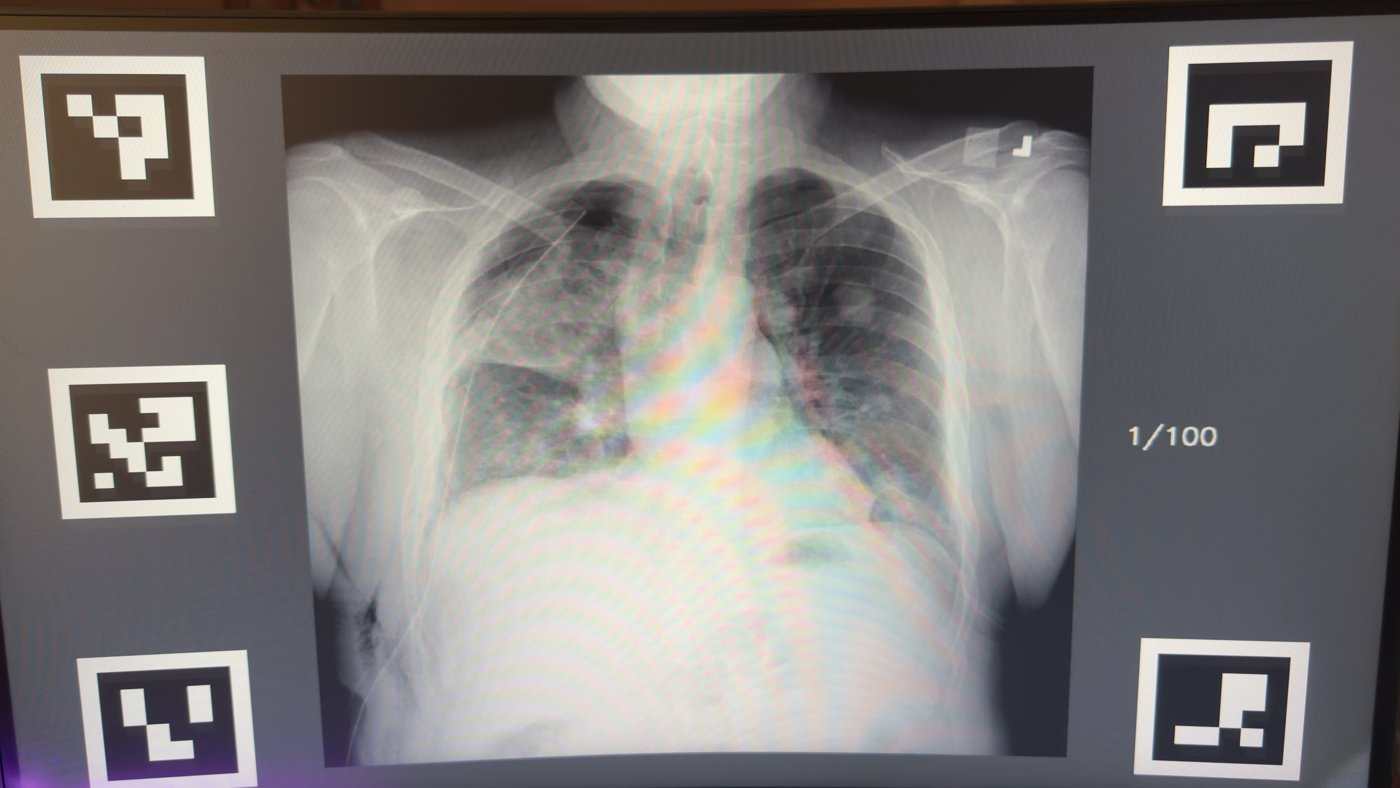
\includegraphics[width=\textwidth]{figs/foto_inclinada.jpg}\\
\nota{iPhone 16 Pro inclinado: marcas ArUco $\to$ homografía $\to$ recorte.}

\vspace{0.4em}
\small AUC: ambos pierden 0.02--0.03.
\end{column}
\begin{column}{0.57\textwidth}
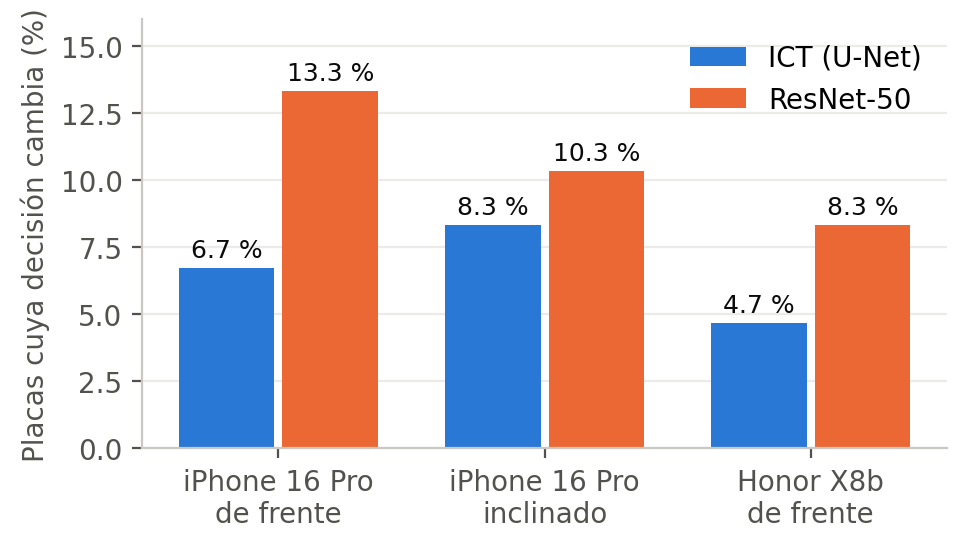
\includegraphics[width=\textwidth]{figs/fotos_cambios.png}
\begin{itemize}\small
\item El \M{ICT} cambia de decisión solo cerca del umbral: mediana a \textbf{0.013} de 0.50 (0.056 en todas).
\item Las degradaciones sintéticas \emph{subestimaron} el efecto real.
\end{itemize}
\end{column}
\end{columns}
\end{frame}

\begin{frame}{La aplicación: medir en el celular, sin enviar la imagen}
\bloque{Resultados · implementación}
\begin{columns}[c]
\begin{column}{0.5\textwidth}
\centering
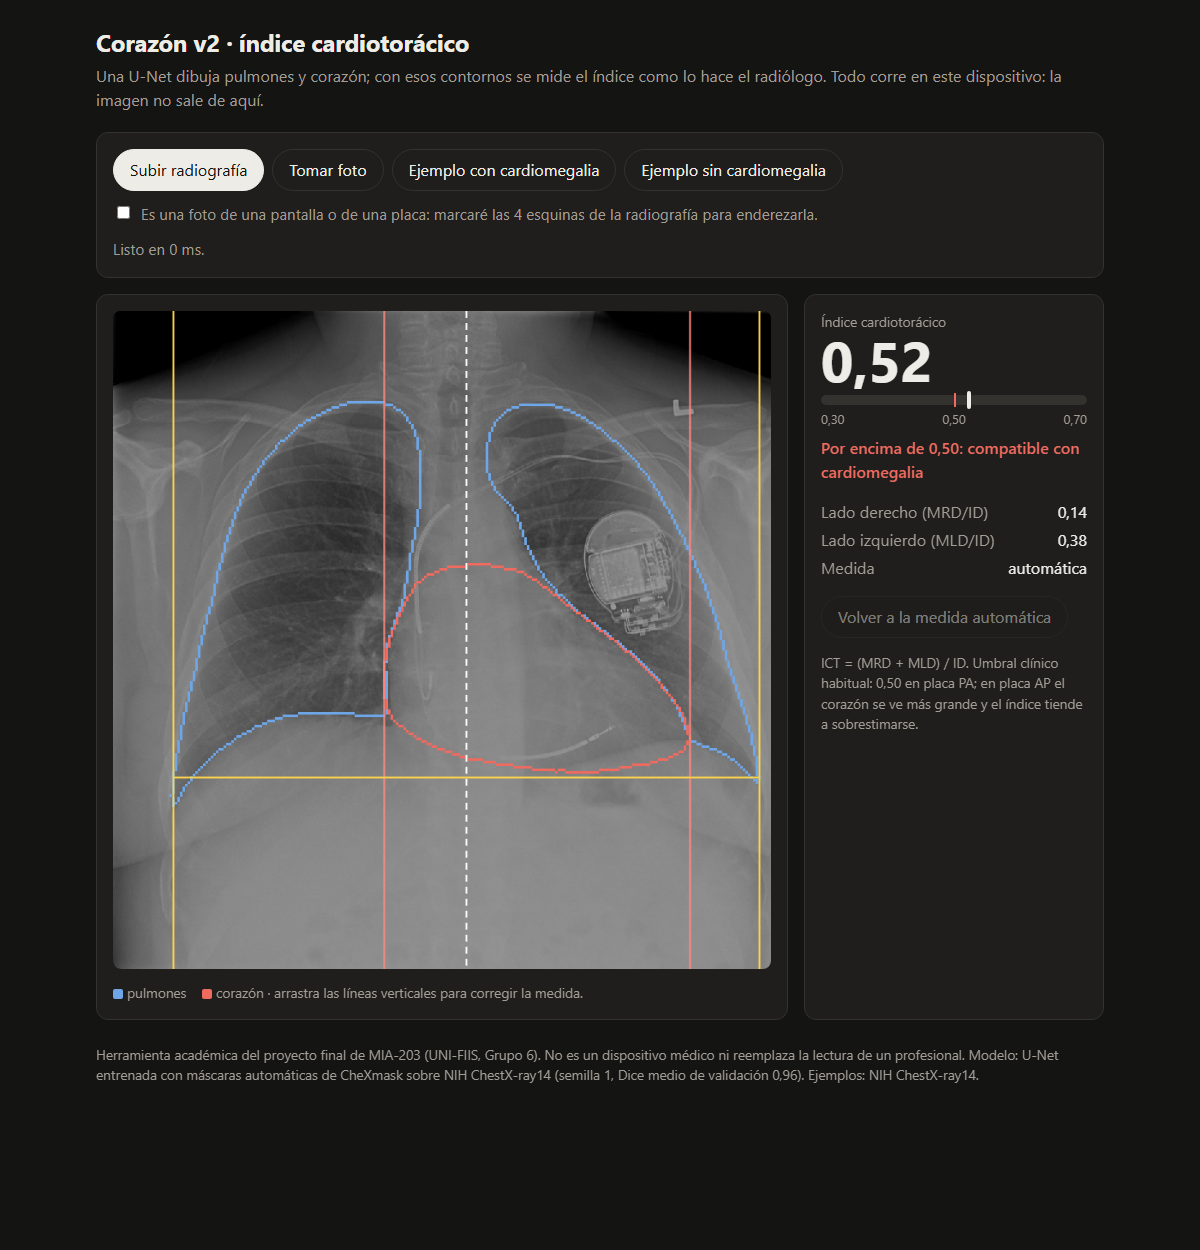
\includegraphics[height=0.78\textheight]{../paper/figs/app.png}
\end{column}
\begin{column}{0.46\textwidth}
\begin{itemize}
\item U-Net exportada a \textbf{ONNX} (31 MB), corre en el navegador.
\item Verificada contra PyTorch: dif.\ máx.\ $2.5\times10^{-6}$; 100\,\% de píxeles iguales; mismo ICT que Python.
\item Para fotos: el usuario marca 4 esquinas y se endereza.
\item Las líneas se \textbf{arrastran}: el médico corrige la medida y el ICT cambia.
\item 1.7--3.2 s por medición en una laptop.
\end{itemize}
\end{column}
\end{columns}
\end{frame}

% ======================================================================================================================
% Bloque 5 — Interpretabilidad, discusión, limitaciones e impacto (4 min)
\begin{frame}{Grad-CAM mira al corazón, también cuando falla}
\bloque{Interpretabilidad}
\begin{columns}[c]
\begin{column}{0.56\textwidth}
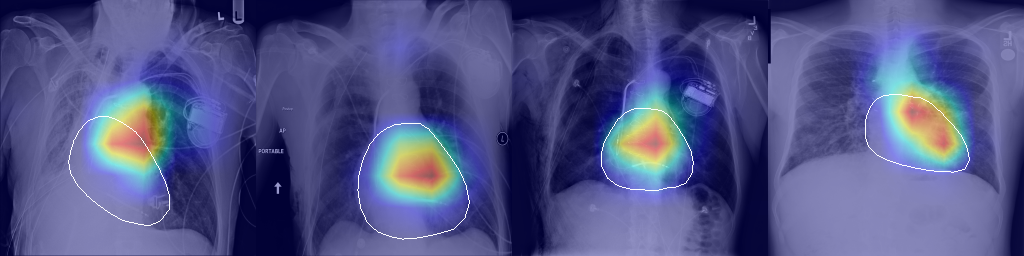
\includegraphics[width=\textwidth]{figs/gradcam_4.png}\\[-0.1em]
\nota{ResNet-50, semilla 0; blanco: corazón de CheXmask. En la 3.ª se ve el rótulo ``PORTABLE'' (vista AP).}\\[0.3em]
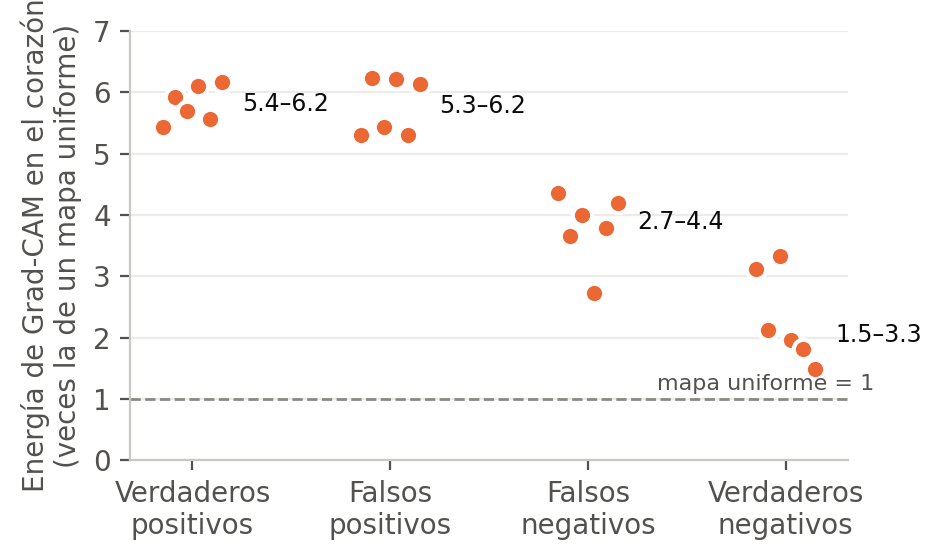
\includegraphics[height=0.42\textheight]{figs/gradcam_grupos.png}
\end{column}
\begin{column}{0.4\textwidth}
\small
\begin{itemize}
\item Energía en el corazón respecto de un mapa uniforme, por grupo (3 semillas × 2 vistas).
\item Falsos positivos = verdaderos positivos (5.3--6.2 vs.\ 5.4--6.2).
\item El mapa dice \emph{dónde} mira, no \emph{si acertó}.
\item Falsos positivos más frecuentes en AP en las 3 semillas.
\end{itemize}
\end{column}
\end{columns}
\end{frame}

\begin{frame}{Discusión: explicar no es lo mismo que medir}
\bloque{Discusión}
\begin{columns}[T]
\begin{column}{0.48\textwidth}
\C{Por qué gana la caja negra}
\begin{itemize}\small
\item Ve toda la placa; el ICT la reduce a un cociente de anchos.
\item La etiqueta del NIH sale del texto del informe, no es ``ICT $>$ 0.50'': las distribuciones se solapan.
\item Aprende de la vista (fuga 0.646): parte de su ventaja puede ser atajo.
\end{itemize}
\end{column}
\begin{column}{0.48\textwidth}
\M{Lo que se gana al medir}
\begin{itemize}\small
\item Errores con nombre: AP $\to$ magnificación $\to$ corrección.
\item Con fotos cambia menos decisiones y solo en casos limítrofes.
\item El error se ve en la placa y se corrige arrastrando una línea.
\end{itemize}
\end{column}
\end{columns}
\vspace{0.6em}
\begin{block}{E6: lo que el ICT frontal no ve}\small
MRD/ID separa peor que MLD/ID (AUC 0.697 vs.\ 0.735). Los falsos negativos no esconden un lado derecho grande: su
MRD/ID (0.138--0.154) es como el de los verdaderos negativos (0.137--0.148). Para el ventrículo derecho haría falta
la placa lateral.
\end{block}
\end{frame}

\begin{frame}{Limitaciones, sesgos e impacto}
\bloque{Responsabilidad}
\begin{columns}[T]
\begin{column}{0.5\textwidth}
\textbf{Limitaciones y sesgos}
\begin{itemize}\small
\item Etiquetas del NIH extraídas por procesamiento de lenguaje: con ruido.
\item Población de EE.\,UU.\ y Japón; sin placas peruanas. Umbral 0.50 de poblaciones de llanura.
\item Fotos de un monitor, no de placas físicas; una sesión, un operador.
\item Referencia dorada: 147 placas JSRT, todas PA.
\end{itemize}
\end{column}
\begin{column}{0.46\textwidth}
\textbf{Impacto y uso responsable}
\begin{itemize}\small
\item Apoyo para una segunda lectura, \textbf{no un diagnóstico} ni un dispositivo médico.
\item La imagen no sale del teléfono.
\item Riesgos: aplicar 0.50 a placas AP sin corregir; sesgo de automatización con la caja negra; usarlo en
  poblaciones no evaluadas.
\item Costo: 4.2 h de GPU T4 para todo el proyecto.
\end{itemize}
\end{column}
\end{columns}
\end{frame}

% ======================================================================================================================
% Bloque 6 — Conclusiones y trabajo futuro (2 min)
\begin{frame}{Conclusiones y trabajo futuro}
\bloque{Conclusiones}
\begin{columns}[T]
\begin{column}{0.52\textwidth}
\begin{itemize}
\item Una U-Net entrenada solo con máscaras automáticas mide el ICT con ICC \M{0.945--0.951} (\M{0.964--0.971} con
  80 contornos humanos).
\item La \C{ResNet-50} detecta mejor (\C{0.892} vs.\ \M{0.814}), pero codifica la vista y cambia más decisiones con
  fotos.
\item El ICT falla de forma \textbf{predecible y corregible}.
\item Sin radiólogo, la elección no es solo de exactitud: es qué error puede revisar quien usa la herramienta.
\end{itemize}
\end{column}
\begin{column}{0.44\textwidth}
\textbf{Trabajo futuro}
\begin{enumerate}\small
\item Validar con placas peruanas e ICT medido por radiólogos; umbral por vista y por altitud.
\item Combinar: ResNet como alerta + ICT como explicación revisable.
\item Esquinas automáticas y fotos de placas físicas.
\item Comparar con HybridGNet y modelos de base tipo Transformer.
\end{enumerate}
\vspace{0.5em}
\nota{Código, resultados y app: github.com/loupv99/corazon-v2}
\end{column}
\end{columns}
\end{frame}

\end{document}
